% !TEX root = ../ui-thesis.tex
% !TeX program = xelatex

\chapter{آموزش مدل و معماری}
\section{معماری کلی پروژه}
در رویکرد ما، هدف این است که مدل‌های جداگانه‌ای برای هر ساز که قصد استفاده در آهنگ خود داریم، آموزش دهیم. به عنوان مثال، ما مدل‌هایی برای پیانو و درام آموزش داده‌ایم. خروجی‌های این مدل‌ها سپس ترکیب می‌شوند تا ترکیب نهایی ایجاد شود و اطمینان حاصل شود که سهم هر ساز به درستی نمایانده شده است.

ورودی مدل‌های ما می‌تواند یک فایل \lr{MIDI} یا هر فایل \lr{WAV} باشد. اگر ورودی یک فایل \lr{WAV} باشد، ابتدا با استفاده از یک الگوریتم تبدیل به نت‌های \lr{MIDI} تبدیل می‌شود. سپس این نت‌های \lr{MIDI} برای پردازش به مدل‌های ما ارسال می‌شوند. این مرحله تبدیل بسیار مهم است زیرا به ما امکان می‌دهد با یک فرمت استاندارد کار کنیم و مدیریت ورودی‌های صوتی مختلف را آسان‌تر می‌کند.

از آنجا که ما از مدل زبان \lr{RWKV} استفاده می‌کنیم، نیاز به یک توکنایزر داریم تا فایل‌های \lr{MIDI} را به فرمت متنی تبدیل کند که مدل بتواند آن را درک کند. توکنایزر فایل‌های \lr{MIDI} را به قطعات کوچکتر و قابل مدیریت تقسیم می‌کند که سپس به مدل \lr{RWKV} تغذیه می‌شوند. این فرآیند به مدل امکان می‌دهد تا به طور مؤثر توالی‌های موسیقی را یاد بگیرد و تولید کند.

\begin{figure}[!htb]
      \centering
      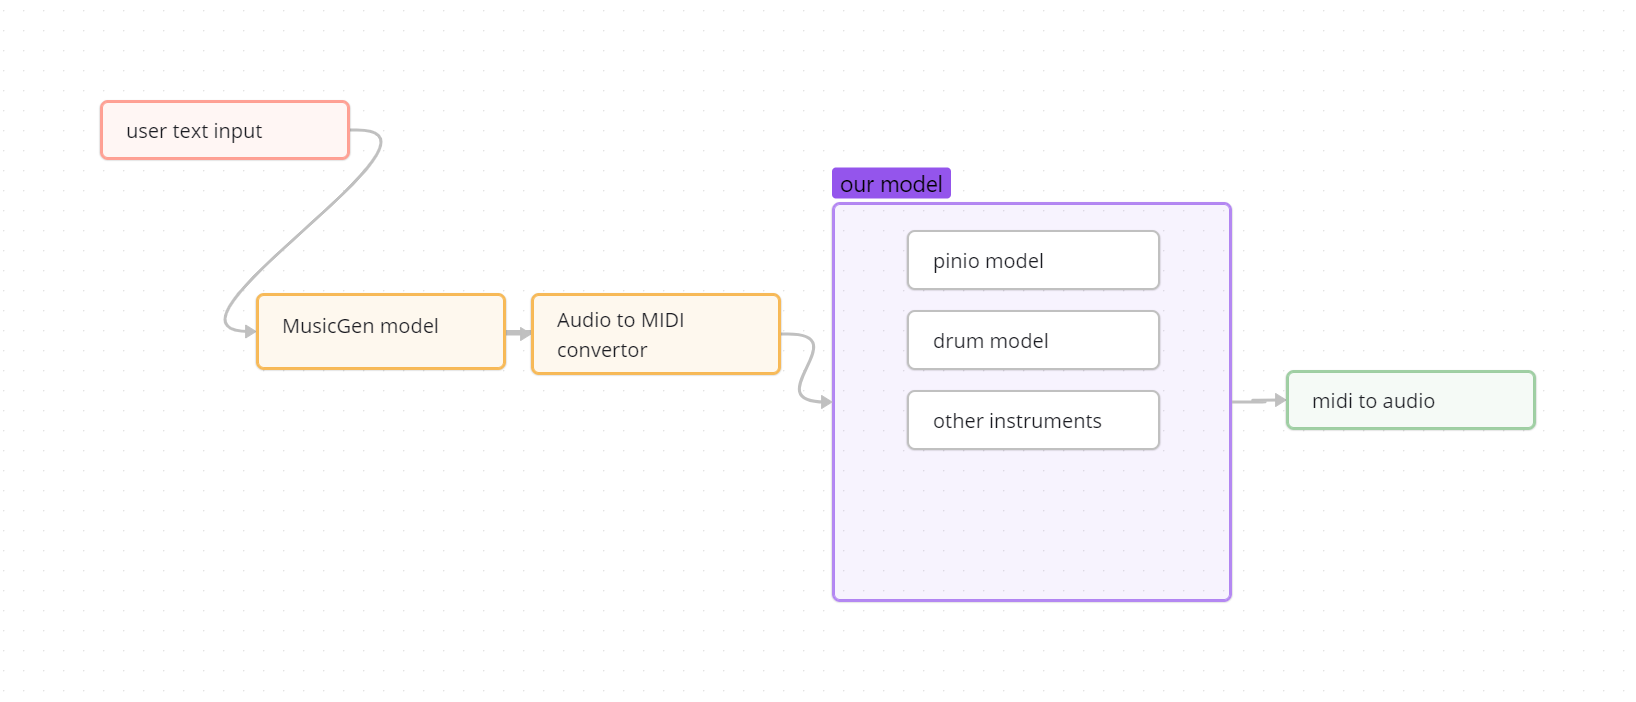
\includegraphics[scale=0.3]{Figures/pipe.png}
      \caption{ساختار  \lr{pipeline}
      }
      \label{Fig:Pipe}
\end{figure}


علاوه بر آموزش مدل‌ها، ما یک  \lr{pipeline} توسعه داده‌ایم که تجربه کاربری را بهبود می‌بخشد. این خط لوله همانطور که در \ref{Fig:Pipe} نشان داده شده است، ورودی متنی کاربر را دریافت کرده و آن را از طریق یک مدل تولید موسیقی \lr{(MusicGen)} \cite{copet2023simple} پردازش می‌کند. مدل \lr{MusicGen} یک فایل \lr{MIDI} بر اساس ورودی متنی کاربر ایجاد می‌کند. این فایل \lr{MIDI} تولید شده سپس از طریق مدل‌های آموزش دیده ما برای هر ساز عبور می‌کند. در نهایت، خروجی این مدل‌ها ترکیب شده و به عنوان ترکیب نهایی موسیقی ذخیره می‌شود.

با آموزش مدل‌های جداگانه برای هر ساز و ترکیب خروجی‌های آن‌ها، می‌توانیم به یک ترکیب موسیقیایی دقیق‌تر و پویا‌تر دست یابیم. این روش انعطاف‌پذیری و خلاقیت بیشتری در تولید موسیقی فراهم می‌کند، زیرا هر ساز می‌تواند به صورت جداگانه تنظیم شود و سپس در قطعه نهایی ادغام شود.

\section{دیتاسیت ها}
\subsubsection{مدل پیانو}

برای انجام آموزش مدل پیانو خود، ما از مجموعه داده گسترده‌ای به نام مجموعه داده \lr{MIDI} موسیقی ایرلندی \lr{IrishMMD} \cite{DBLP:conf/hcmir/WuLY023} استفاده کردیم. این مجموعه داده شامل 216,284 قطعه موسیقی ایرلندی به فرمت \lr{MIDI} است. این مجموعه داده به دو بخش تقسیم شده است: 99\% (214,122 قطعه) برای آموزش مدل و \%1 (2,162 قطعه) برای ارزیابی آن.

قطعات موسیقی این مجموعه داده از وب‌سایت‌های \lr{thesession.org} و \lr{abcnotation.com} جمع‌آوری شده‌اند. برای اطمینان از یکپارچگی داده‌ها، ممکن است برخی از قطعات موسیقی که به صورت متن بودند به فرمت \lr{MIDI} تبدیل شده باشند. همچنین، اطلاعات غیرموسیقی مانند عنوان و متن ترانه‌ها حذف شده است.
\subsubsection{مدل دارم}
\textbf{مجموعه داده گسترده \lr{EGMD} \cite{callender2020improving}}

برای تحقیق خود، ما از نسخه گسترده‌تری از مجموعه داده \lr{EGMD}
استفاده کردیم که به عنوان \textbf{مجموعه داده گسترده \lr{EGMD}}
شناخته می‌شود. \lr{GMD} یک مجموعه داده از اجراهای درام انسانی است که به صورت
\lr{MIDI} بر روی یک درام کیت الکترونیکی \lr{Roland TD-11} ضبط شده است.

\begin{table}[!ht]
      \centering
      \begin{tabular}{|l|l|l|l|}
            \hline
            بخش        & تعداد توالی‌های منحصربه‌فرد & تعداد کل توالی‌ها & مدت زمان (ساعت) \\ \hline
            آموزشی     & 819                       & 35,217           & 341.4           \\ \hline
            آزمایشی    & 123                       & 5,289            & 50.9            \\ \hline
            اعتبارسنجی & 117                       & 5,031            & 52.2            \\ \hline
            کل         & 1,059                     & 45,537           & 444.5           \\ \hline
      \end{tabular}
      \caption{خلاصه‌ای از مجموعه داده}
      \label{drumInfo}
\end{table}

ما تقسیم‌بندی‌های آموزشی، آزمایشی و اعتبارسنجی را که در \lr{GMD} وجود داشت، حفظ
کردیم. نکته مهم این است که از آنجایی که هر کیت برای هر توالی ضبط شده
است، تمام 43 کیت در بخش‌های آموزشی، آزمایشی و اعتبارسنجی وجود دارند. که به طور خلاصه در \ref{drumInfo} نشان داده شده است.


\section{تبدیل \lr{MIDI} به متن}\label{se:tokenizer}

\subsection{رویکرد های موجود برای توکن‌سازی فایل‌های \lr{MIDI}}

در نمایش موسیقی به متن، چندین فرمت مختلف وجود دارد که می‌توان برای نمایش اطلاعات
موسیقی استفاده کرد. یکی از رایج‌ترین فرمت‌ها، نوت‌نویسی \lr{ABC} است
که یک فرمت قابل خواندن توسط انسان است و موسیقی را با استفاده از ترکیبی
از حروف و نمادها برای نشان دادن ارتفاع صدا، مدت زمان و سایر عناصر موسیقی
نمایش می‌دهد. نوت‌نویسی \lr{ABC} به طور گسترده‌ای در نظریه موسیقی و آموزش موسیقی
استفاده می‌شود.

با این حال، برای آموزش یک مدل زبانی برای تولید موسیقی
لو-فای، باید تعادل بین پیچیدگی داده‌های ورودی و توانایی مدل در
یادگیری از آن‌ها را در نظر بگیریم. در این مورد، ما تصمیم گرفتیم فایل‌های
\lr{MIDI} را به فرمت \lr{MIDICompact} توکن‌سازی کنیم که یک نمایش ساده‌تر از
اطلاعات موسیقی است.

فرمت \lr{MIDICompact}

در فرمت \lr{MIDICompact}، هر توکن یک رویداد موسیقی را نشان می‌دهد که
ساختار آن به شرح زیر است:

در اینجا تجزیه و تحلیل اجزای فرمت آمده است:
اگر یک نوت را به صورت
\begin{LTR}
      \begin{verbatim}
            <Note>:<velocity> <Wait time>
      \end{verbatim}
\end{LTR}
در نظر بگیریم خواهیم داشت

\begin{itemize}
      \item[\lr{<Note>}]
            این نشان دهنده نوتی است که نواخته می‌شود، جایی که \lr{<Note>} یک مقدار هگزادسیمال بین 0 و 25 است. در این نمایش، هر نوت یک مقدار هگزادسیمال منحصر به فرد دارد که در \xt{noteMap} نشان داده شده است.
      \item[\lr{<velocity>}]  این یک جداکننده بین نوت و شدت صدا است.\footnote{در اینجا برای سادگی از 25 نوت استفاده شده ولی در کد های نوشته شده از 128 نوت استفاده شده که کیفیت یادگیری را افزایش می‌دهد.}
            این نشان دهنده شدت صدای نوت است، جایی که \lr{<velocity>} یک مقدار هگزادسیمال بین 0 و 15 است. شدت صدا به 16 مقدار ممکن تقسیم می‌شود که در \xt{velSpeed} نشان داده شده است.
      \item[ \lr{<Wait time>}]
            این نشان دهنده یک توکن انتظار است که نشان می‌دهد چه مدت باید قبل از نواختن نوت بعدی صبر کرد. توکن انتظار به صورت یک مقدار دهدهی بین 1 و 100 نمایش داده می‌شود، جایی که 1 نشان دهنده زمان انتظار بسیار کوتاه و 100 نشان دهنده زمان انتظار بسیار طولانی است.
\end{itemize}

\begin{table}%
      \centering
      \subfloat[\centering نگاشت نوت ها ]{
            \begin{tabular}{|c|c|}
                  \hline
                  \textbf{\lr{Hex}} & \textbf{نوت} \\
                  \hline
                  0                 & \lr{A0}      \\
                  1                 & \lr{A\#}     \\
                  2                 & \lr{B}       \\
                  3                 & \lr{C}       \\
                  4                 & \lr{C\#}     \\
                  5                 & \lr{D}       \\
                  6                 & \lr{D\#}     \\
                  7                 & \lr{E}       \\
                  8                 & \lr{F}       \\
                  9                 & \lr{F\#}     \\
                  10                & \lr{G}       \\
                  11                & \lr{G\#}     \\
                  12                & \lr{A}       \\
                  13                & \lr{A\#}     \\
                  14                & \lr{B}       \\
                  15                & \lr{C}       \\
                  16                & \lr{C\#}     \\
                  17                & \lr{D}       \\
                  18                & \lr{D\#}     \\
                  19                & \lr{E}       \\
                  20                & \lr{F}       \\
                  21                & \lr{F\#}     \\
                  22                & \lr{G}       \\
                  23                & \lr{G\#}     \\
                  24                & \lr{A}       \\
                  25                & \lr{B}       \\
                  \hline
            \end{tabular}
      }%
      \qquad
      \subfloat[\centering  نگاشت سرعت ]{
            \begin{tabular}{|c|c|}
                  \hline
                  \textbf{\lr{Hex}} & \textbf{\lr{سرعت}}        \\
                  \hline
                  0                 & 0-10\% (بسیار نرم)        \\
                  1                 & 11-20\% (نرم)             \\
                  2                 & 21-30\% (نسبتاً نرم)       \\
                  3                 & 31-40\% (متوسط)           \\
                  4                 & 41-50\% (نسبتاً سخت)       \\
                  5                 & 51-60\% (سخت)             \\
                  6                 & 61-70\% (بسیار سخت)       \\
                  7                 & 71-80\% (بسیار بسیار سخت) \\
                  8                 & 81-90\% (حداکثر)          \\
                  9                 & 91-100\% (حداکثر)         \\
                  10                & 101-110\% (حداکثر)        \\
                  11                & 111-120\% (حداکثر)        \\
                  12                & 121-130\% (حداکثر)        \\
                  13                & 131-140\% (حداکثر)        \\
                  14                & 141-150\% (حداکثر)        \\
                  15                & 151-160\% (حداکثر)        \\
                  \hline
            \end{tabular}
      }%
      \caption{نگاشت های فرمت \lr{MIDICompact}}
      \label{tb:MIDICompact}%
\end{table}


این فرمت اجازه می‌دهد تا اطلاعات موسیقی به صورت فشرده و کارآمد نمایش داده
شود، که آن را برای استفاده در پروژه ما به خوبی عمل کند. تعداد کل توکن هایی که می‌تواند ساخته شود به صورت زیر است:

$ (Note * velocity) + Wait  time + pad + start + end =(128 * 16) + 125 + 3 = 2176$
\begin{example}[]
      \centering
      \label{example:token}
      برای مثال \texttt{<start> 3:5 t1  10:2 t2  1:14 t5  d:11 t3 <end>} می تواند خروجی الگوریتم \ref{alg:token} باشد.

      \lr{A} (نوت 3) با شدت صدای 5 (نسبتاً سخت) و زمان انتظار 1

      \lr{C\#} (نوت 10) با شدت صدای 2 (نسبتاً نرم) و زمان انتظار 2

      \lr{B} (نوت 1) با شدت صدای 14 (حداکثر) و زمان انتظار 5

      \lr{A\#} (نوت 13) با شدت صدای 11 (بسیار بسیار سخت) و زمان انتظار 3
\end{example}

در حالی که فرمت \lr{ABC} بیانگرتر است و می‌تواند طیف گسترده‌ای از ظرافت‌های
موسیقی را نمایش دهد، همچنین پیچیدگی اضافی را معرفی می‌کند  که ممکن است
برای پروژه ما ضروری نیست. به ویژه، فرمت \lr{ABC} نیاز دارد که مدل تعداد
بیشتری از توکن‌ها و روابط بین آن‌ها را یاد بگیرد که می‌تواند منجر به
بیش‌برازش و کاهش قابلیت تعمیم‌دهی شود.

در تولید موسیقی، مقادیر سرعت \LTRfootnote{velocity} اغلب پیوسته هستند، اما
در تولید صدا که در  \xs{finalMusic} توضیح داده شده است، تنها می‌تواند مقادیر گسسته تولید کند. با کوانتایز کردن
مقادیر سرعت به تعداد ثابتی از بین‌ها \LTRfootnote{bins}، سیستم می‌تواند خروجی‌ای
سازگارتر و قابل پیش‌بینی‌تر تولید کند. این روش به‌ویژه در موسیقی لو-فای
مفید است، جایی که هدف ایجاد صدایی سازگار است. کد یک تابع
کوانتایز کردن سرعت را پیاده‌سازی می‌کند که می‌تواند خطی یا نمایی باشد. این
تابع یک مقدار سرعت پیوسته را به یک بین گسسته نگاشت می‌کند، که یک تکنیک
رایج در تولید موسیقی، به‌ویژه در موسیقی لو-فای است.

\subsubsection{کوانتایز کردن
      خطی}

در کوانتایز کردن خطی، مقدار سرعت پیوسته به تعداد ثابتی از بین‌های گسسته
تقسیم می‌شود. اندازه بین با تقسیم حداکثر مقدار سرعت بر تعداد بین‌ها تعیین
می‌شود. شاخص بین با تقسیم مقدار سرعت بر اندازه بین و گرد کردن به
نزدیک‌ترین عدد صحیح محاسبه می‌شود.

\subsubsection{کوانتایز کردن
      نمایی}
در کوانتایز کردن نمایی، مقدار سرعت پیوسته با استفاده از یک تابع نمایی به
یک بین گسسته نگاشت می‌شود. تابع نمایی توسط پارامتر \lr{velocity\_exp} کنترل
می‌شود که شکل منحنی را تعیین می‌کند. مقدار بالاتر \lr{velocity\_exp} منجر به
منحنی نمایی‌تر می‌شود، در حالی که مقدار پایین‌تر منجر به منحنی خطی‌تر می‌شود.

\subsubsection{ریاضیات پشت کوانتایز کردن
      نمایی}

فرمول کوانتایز کردن نمایی به صورت زیر است:
\begin{LTR}
      \setmainfont{Times New Roman}
      $
            \text{bin\_index} = \lceil \frac{\text{velocity\_events} \cdot (\exp(\frac{\text{velocity}}{\text{velocity\_events}}) - 1)}{\exp(1) - 1} \rceil
      $
\end{LTR}
که در آن \lr{velocity\_events} حداکثر مقدار سرعت، \lr{velocity} مقدار سرعت ورودی و
\lr{exp} تابع نمایی است.

\subsubsection{چرا کوانتایز کردن
      نمایی؟}
کوانتایز کردن نمایی در تولید موسیقی بهتر است زیرا اجازه می‌دهد صدایی
ظریف‌تر و دقیق‌تر ایجاد شود. در این پروژه ما مقدار پارامتر \lr{velocity\_exp} را برابر $0.33$ قرار دادیم.

\begin{LTR}
      \begin{algorithm}
            \caption{کوانتایز کردن سرعت}
            \label{alg:velocity_quantization}
            \begin{algorithmic}
                  \setmainfont{Times New Roman}
                  \Procedure{velocity\_to\_bin}{velocity}
                  \State $bin\_size \gets \frac{\text{velocity\_events}}{\text{velocity\_bins} - 1}$
                  \If{$\text{velocity\_exp} == 1.0$}
                  \State $bin \gets \lceil \frac{\text{velocity}}{bin\_size} \rceil$
                  \Else
                  \State $bin \gets \lceil \left( \text{velocity\_events} \cdot \left( \left( \text{velocity\_exp}^{ \frac{\text{velocity}}{\text{velocity\_events}} } - 1 \right) \right) / (\text{velocity\_exp} - 1) \right) / bin\_size \rceil$
                  \EndIf
                  \State \Return $bin$
                  \EndProcedure

                  \Procedure{bin\_to\_velocity}{bin}
                  \State $bin\_size \gets \frac{\text{velocity\_events}}{\text{velocity\_bins} - 1}$
                  \If{$\text{velocity\_exp} == 1.0$}
                  \State $velocity \gets \max(0, \lceil bin \cdot bin\_size - 1 \rceil)$
                  \Else
                  \State $velocity \gets \max(0, \lceil \text{velocity\_events} \cdot \log \left( \frac{(\text{velocity\_exp} - 1) \cdot bin \cdot bin\_size}{\text{velocity\_events}} + 1, \text{velocity\_exp} \right) - 1 \rceil)$
                  \EndIf
                  \State \Return $velocity$
                  \EndProcedure
            \end{algorithmic}
      \end{algorithm}
\end{LTR}


توضیحات \xal{alg:token} که به تبدیل داده ها به متن می‌کند به صورت زیر است:
\begin{itemize}
      \item {پیش‌پردازش}
            \begin{itemize}
                  \item
                        \textbf{فیلتر کردن}: حذف پیام‌های متا ناشناخته برای اطمینان از پردازش
                        فقط داده‌های \lr{MIDI} مرتبط.
                  \item
                        \textbf{ادغام ترک‌ها}: اگر فایل \lr{MIDI} شامل چندین ترک باشد، آن‌ها را به یک
                        ترک واحد ادغام کنید تا پردازش ساده‌تر شود.
            \end{itemize}

      \item {مدیریت وضعیت}

            \begin{itemize}

                  \item
                        \textbf{وضعیت کانال‌ها}: نگهداری دیکشنری‌هایی برای پیگیری وضعیت هر کانال
                        \lr{MIDI} شامل تغییرات برنامه، حجم، بیان، نوت‌های فعال و وضعیت پدال.
                  \item
                        \textbf{زمان‌بندی}: پیگیری زمان سپری شده بین رویدادهای \lr{MIDI} برای نمایش
                        دقیق زمان‌بندی در توالی توکن‌ها.
            \end{itemize}

      \item {بافر  توکن}

            \begin{itemize}

                  \item
                        \textbf{بافرینگ}: استفاده از یک بافر برای ذخیره موقت داده‌های توکن قبل
                        از تبدیل آن‌ها به توکن‌های رشته‌ای. این کار به مدیریت زمان‌بندی و توالی
                        توکن‌ها کمک می‌کند.
            \end{itemize}

      \item {پردازش رویدادها}

            \begin{itemize}

                  \item
                        \textbf{رویدادهای نوت}: پردازش رویدادهای \texttt{note\_on} و
                        \texttt{note\_off} برای شروع و توقف نوت‌ها، با در نظر گرفتن سرعت، حجم و
                        بیان.
                  \item
                        \textbf{تغییرات کنترل}: پردازش پیام‌های تغییر کنترل برای به‌روزرسانی
                        وضعیت کانال‌ها، مانند حجم، بیان و وضعیت پدال.
            \end{itemize}

      \item    {تولید توکن}

            \begin{itemize}

                  \item
                        \textbf{تبدیل توکن}: تبدیل داده‌های نوت بافر شده به توکن‌های رشته‌ای با
                        استفاده از فرمت‌های از پیش تعریف شده. این شامل نگاشت رویدادهای \lr{MIDI} به
                        نمایش‌های خاص توکن است.
                  \item
                        \textbf{توکن‌های زمان‌بندی}: تولید توکن‌هایی که زمان سپری شده بین
                        رویدادها را نمایش می‌دهند تا ساختار زمانی موسیقی حفظ شود.
            \end{itemize}

      \item{ساخت خروجی}

            \begin{itemize}

                  \item
                        \textbf{تقسیم قطعات}: تقسیم خروجی به قطعات بر اساس سکوت یا معیارهای
                        دیگر برای ایجاد بخش‌های قابل مدیریت از توکن‌ها.
                  \item
                        \textbf{نهایی‌سازی}: افزودن توکن‌های شروع و پایان به هر قطعه و ترکیب
                        لیست نهایی توالی‌های توکن.
            \end{itemize}

\end{itemize}

این رویکرد شامل پیش‌پردازش داده‌های \lr{MIDI}، مدیریت وضعیت کانال‌های \lr{MIDI}، بافر
کردن داده‌های توکن، پردازش رویدادهای مختلف \lr{MIDI}، تولید توکن‌ها و ساخت
خروجی نهایی است. این روش اطمینان می‌دهد که ساختار زمانی و موسیقیایی فایل
\lr{MIDI} به‌طور دقیق در توالی توکن‌ها نمایش داده می‌شود.

\begin{LTR}
      \begin{algorithm}
            \caption{توکن کردن فایل های \lr{MIDI}}
            \label{alg:token}
            \setmainfont{Times New Roman}
            \begin{algorithmic}[1]
                  \Function{convert\_midi\_to\_str}{cfg, filter\_cfg, mid, augment=None}
                  \State Initialize state variables

                  \Function{flush\_token\_data\_buffer}{}
                  \State Convert token data buffer to token data
                  \State Append formatted tokens to output
                  \State Clear token data buffer
                  \EndFunction

                  \Function{consume\_note\_program\_data}{prog, chan, note, vel}
                  \If{token is valid}
                  \If{delta\_time\_ms $>$ threshold}
                  \State Check if any notes are held
                  \If{no notes are held}
                  \State Call \textproc{flush\_token\_data\_buffer}()
                  \State Append "<end>" to output
                  \State Reset output and state variables
                  \EndIf
                  \EndIf
                  \State Generate wait tokens and append to output
                  \State Reset delta\_time\_ms
                  \State Append token data to buffer
                  \State Set started\_flag to True
                  \EndIf
                  \EndFunction

                  \For{each msg in mid.tracks[0]}
                  \State Update delta\_time\_ms with msg.time

                  \Function{handle\_note\_off}{ch, prog, n}
                  \If{pedal is on}
                  \State Set pedal event
                  \Else
                  \State Call \textproc{consume\_note\_program\_data}(prog, ch, n, 0)
                  \State Remove note from channel\_notes
                  \EndIf
                  \EndFunction

                  \If{msg.type is "program\_change"}
                  \State Update channel\_program
                  \ElsIf{msg.type is "note\_on"}
                  \If{velocity is 0}
                  \State Call \textproc{handle\_note\_off}
                  \Else
                  \State Remove pedal event if exists
                  \State Call \textproc{consume\_note\_program\_data} with mixed volume
                  \State Add note to channel\_notes
                  \EndIf
                  \ElsIf{msg.type is "note\_off"}
                  \State Call \textproc{handle\_note\_off}
                  \ElsIf{msg.type is "control\_change"}
                  \State Update channel state based on control type
                  \Else
                  \State \textbf{pass}
                  \EndIf
                  \EndFor

                  \State Call \textproc{flush\_token\_data\_buffer}()
                  \State Append "<end>" to output
                  \State \Return output\_list
                  \EndFunction
            \end{algorithmic}
      \end{algorithm}
\end{LTR}



\subsection{توکن سازی}

در کار ما، از یک رویکرد ساده برای آماده‌سازی و آموزش مدل با استفاده از
کتابخانه \lr{Tokenizer} \cite{Moi_HuggingFace_s_Tokenizers_2023} استفاده کردیم. در اینجا توضیح دقیقی از این فرآیند
آورده شده است:

\subsubsection{توکن‌سازی سریع با کتابخانه \lr{Tokenizer}}

ما از کتابخانه \lr{Tokenizer} برای انجام توکن‌سازی سریع و کارآمد داده‌ها
استفاده کردیم. این کتابخانه برای پردازش مجموعه داده‌های بزرگ و تبدیل متن
خام به توکن‌ها به سرعت طراحی شده است. مزایای کلیدی استفاده از این
کتابخانه شامل موارد زیر است: - \textbf{سرعت}: کتابخانه \lr{Tokenizer} برای
عملکرد بهینه‌سازی شده است و به ما امکان می‌دهد حجم زیادی از داده‌ها را در
زمان کوتاهی پردازش کنیم. - \textbf{انعطاف‌پذیری}: این کتابخانه از
استراتژی‌های مختلف توکن‌سازی پشتیبانی می‌کند و به راحتی می‌توان آن را برای
نیازهای خاص پروژه سفارشی کرد.

\subsubsection{تبدیل به فرمت \lr{JSONL}}

پس از توکن‌سازی، داده‌های توکن‌شده را به فرمت \lr{JSON Lines (JSONL)} تبدیل
کردیم. این فرمت به خصوص برای پردازش مجموعه داده‌های بزرگ مناسب است زیرا:
- \textbf{پردازش خط به خط}: هر خط در یک فایل \lr{JSONL} نمایانگر یک شیء \lr{JSON}
جداگانه است که پردازش داده‌ها را خط به خط بدون نیاز به بارگذاری کل مجموعه
داده در حافظه آسان می‌کند. - \textbf{سادگی}: \lr{JSONL} به راحتی خوانده و
نوشته می‌شود و با بسیاری از ابزارهای پردازش داده‌ها به خوبی ادغام می‌شود.

\subsubsection{تبدیل به فرمت \lr{binidx} برای آموزش سریع}

برای بهینه‌سازی بیشتر فرآیند آموزش، داده‌های \lr{JSONL} را به فرمت \lr{binidx} تبدیل
کردیم. \lr{binidx} یک فرمت باینری است که چندین مزیت برای آموزش مدل‌های یادگیری
ماشین ارائه می‌دهد: - \textbf{کارایی}: فرمت‌های باینری به طور کلی فشرده‌تر
و سریع‌تر برای خواندن/نوشتن نسبت به فرمت‌های متنی هستند و سربار \lr{I/O} را در
طول آموزش کاهش می‌دهند. - \textbf{سازگاری}: فرمت \lr{binidx} با بسیاری از
چارچوب‌های یادگیری ماشین سازگار است و ادغام بدون مشکل در خط لوله آموزش ما
را تسهیل می‌کند. ما برای تبدیل فایل های \lr{JSONL} به فرمت \lr{binidx} از بخشی از کد های کتابخانه \lr{gpt-neox} \cite{gpt-neox-library} استفاده کردیم.

با استفاده از کتابخانه \lr{Tokenizer} برای توکن‌سازی سریع و تبدیل داده‌ها به
فرمت \lr{JSONL} و سپس به فرمت \lr{binidx}، ما به طور قابل توجهی کارایی فرآیندهای
آماده‌سازی داده و آموزش را بهبود بخشیدیم. این رویکرد به ما امکان داد تا
مجموعه داده‌های بزرگ را به طور مؤثر مدیریت کنیم و زمان کلی آموزش را تسریع
کنیم که منجر به توسعه کارآمدتر مدل شد.

\section{آموزش مدل}
\subsection{پارامترهای آموزش مدل}
در این بخش، پارامترهای مورد استفاده برای آموزش مدل توضیح داده شده‌اند:

ما از معماری \texttt{rwkv-6.0} \cite{peng2024eagle} استفاده کردیم. همچنین
امکان استفاده از مدل دارد. مدل ما شامل 20 لایه و
\lr{embedding} برابر با 512 است. \lr{Context Length} \footnote{\lr{Context Length} بی‌نهایت فقط در هنگام اجرای مدل معنا می  دهد.} مدل برابر با
512 است.
مقدار نرخ یادگیری اولیه و نهایی برابر با \num{6e-4}   و \num{6e-5} است.

\subsection{نحویه آموزش مدل}
\begin{LTR}

      \begin{algorithm}
            \caption{آموزش مدل}
            \label{alg:Training}
            \setmainfont{Times New Roman}
            \begin{algorithmic}[1]
                  \State \textbf{Function} save\_pth(dd, ff)
                  \State torch.save(dd, ff)

                  \State \textbf{Class} ResetValDataloader(Callback)
                  \State \textbf{Function} on\_validation\_start(trainer, pl\_module)
                  \State trainer.reset\_val\_dataloader(pl\_module)

                  \State \textbf{Class} TrainCallback(Callback)
                  \State \textbf{Function} \_\_init\_\_(self, args)
                  \State self.args = args

                  \State \textbf{Function} on\_train\_batch\_start(self, trainer, pl\_module, batch, batch\_idx)
                  \State Adjust learning rate based on global step and schedule
                  \For{param\_group \textbf{in} trainer.optimizers[0].param\_groups}
                  \State param\_group['lr'] = lr * param\_group['my\_lr\_scale'] \textbf{if} args.layerwise\_lr > 0 \textbf{else} lr
                  \EndFor
                  \State trainer.my\_lr = lr

                  \State \textbf{Function} on\_train\_batch\_end(self, trainer, pl\_module, outputs, batch, batch\_idx)
                  \State Log metrics and update loss

                  \State \textbf{Function} on\_train\_epoch\_start(self, trainer, pl\_module)
                  \State Update dataset attributes

                  \State \textbf{Function} on\_train\_epoch\_end(self, trainer, pl\_module)
                  \If{trainer.is\_global\_zero \textbf{and} (args.epoch\_save > 0 \textbf{and} trainer.current\_epoch \% args.epoch\_save == 0) \textbf{or} (trainer.current\_epoch == args.epoch\_count - 1)}
                  \State save\_pth(pl\_module.state\_dict(), f'{args.proj\_dir}/{self.prefix}\_{args.epoch\_begin + trainer.current\_epoch}.pth')
                  \EndIf
            \end{algorithmic}
      \end{algorithm}
\end{LTR}
\xal{alg:Training}  برای مدیریت و بهینه‌سازی فرآیند آموزش  مدل
با استفاده از \lr{PyTorch Lightning} \cite{Falcon_PyTorch_Lightning_2019}
طراحی شده است.

ابتدا، تابع \texttt{save\_pth}  که برای ذخیره دیکشنری حالت
مدل در یک مسیر فایل مشخص استفاده می‌شود. این قابلیت برای ایجاد نقاط
بازرسی در طول آموزش ضروری است و به مدل اجازه می‌دهد تا ذخیره و بعداً
بارگذاری شود. این امر تضمین می‌کند که فرآیند آموزش می‌تواند از آخرین حالت
ذخیره شده در صورت وقفه‌ها از سر گرفته شود و پیشرفت‌های حاصل شده در طول
آموزش حفظ شود.

کلاس \texttt{TrainCallback} با آرگومان‌های مختلفی که فرآیند آموزش را
کنترل می‌کنند، مقداردهی اولیه می‌شود. این شامل تنظیم برنامه‌های نرخ
یادگیری، لاگ‌گیری و سایر پارامترهای خاص آموزش است. در متد
\texttt{on\_train\_batch\_start}، نرخ یادگیری به صورت پویا بر اساس مرحله
فعلی آموزش تنظیم می‌شود. برنامه نرخ یادگیری به دو مرحله اصلی تقسیم می‌شود:
مرحله گرم‌کردن \LTRfootnote{warm up} و مرحله کاهش. در مرحله گرم‌کردن، نرخ یادگیری به تدریج از یک
مقدار کوچک به نرخ یادگیری اولیه افزایش می‌یابد. این کار به فرآیند
آموزش در مراحل اولیه کمک زیادی می‌کند. در مرحله کاهش، نرخ یادگیری بر اساس کاهش
خطی یا نمایی تنظیم می‌شود. این تنظیم پویا نرخ
یادگیری به بهینه‌سازی فرآیند آموزش و بهبود همگرایی کمک می‌کند.

لاگ‌گیری و نظارت گسترده بخش‌های جدایی‌ناپذیر این بخش هستند. متدهای
\texttt{on\_train\_batch\_start} و \texttt{on\_train\_batch\_end} شامل
مکانیزم‌های لاگ‌گیری دقیقی برای دیدن پیشرفت آموزش هستند. این شامل
لاگ‌گیری نرخ یادگیری و \lr{Loss Function}، پیگیری تعداد توکن‌های پردازش شده در هر
ثانیه و لاگ‌گیری به سرویس‌های مانند \lr{Weights \& Biases (wandb)} \cite{wandb} برای
پیگیری آزمایش‌ها است.

متدهای \texttt{on\_train\_epoch\_start} و \texttt{on\_train\_epoch\_end}
وظایفی را که باید در ابتدای هر دوره آموزش و پایان آن انجام شوند، مدیریت
می‌کنند. این شامل تنظیم پارامترهای مجموعه داده مانند رتبه جهانی و دوره
واقعی و ذخیره نقاط بازرسی مدل در فواصل مشخص یا در پایان آموزش است. ذخیره
منظم نقاط بازرسی مدل تضمین می‌کند که فرآیند آموزش می‌تواند از آخرین حالت
ذخیره شده از سر گرفته شود و یک محافظت در برابر وقفه‌ها فراهم می‌کند.

\subsubsection{کتابخانه‌ها استفاده شده}
چندین کتابخانه در این روش برای ساده‌سازی فرآیند آموزش استفاده می‌شوند.
کتابخانه \texttt{torch} \cite{paszke2017automatic}  قابلیت‌های اصلی برای ساخت و آموزش
شبکه‌های عصبی را فراهم می‌کند. \lr{PyTorch Lightning} \cite{Falcon_PyTorch_Lightning_2019} فرآیند آموزش را با انتزاع
کدهای تکراری ساده می‌کند، حلقه‌های آموزش، اعتبارسنجی و تست را از طریق کلاس
\texttt{Trainer} مدیریت می‌کند و از کلاس‌های \texttt{Callback} برای افزودن
رفتار سفارشی در مراحل مختلف آموزش استفاده می‌کند. کتابخانه \texttt{wandb}
برای لاگ‌گیری و پیگیری آزمایش‌ها استفاده می‌شود.

\section{ارزیابی عملکرد مدل}
\subsection{ارزیابی مدل پیانو}

با توجه به \xf{Fig:lrpi} می توان گفت که مدل سبز \footnote{در اینجا مدل سبز به مدل  \lr{ctx512 L20 D512} اشاره می‌کند. که مدل نهایی انتخاب شده برای ارزیابی است.} به دلیل شروع با مقدار اولیه کمتری از خطا، عملکرد بهتری دارد. این موضوع می‌تواند به دلیل پیش‌آموزش مؤثرتر یا وزن‌های اولیه بهتر باشد. برخلاف مدل‌های قرمز و آبی که کاهش سریعی در خطا نشان می‌دهند و سپس به یک سطح ثابت می‌رسند، مدل سبز به تدریج و به طور پیوسته کاهش می‌یابد. این نشان‌دهنده یک فرآیند یادگیری پایدارتر است که خطر بیش‌برازش را کاهش می‌دهد و اطمینان می‌دهد که مدل به داده‌های جدید بهتر تعمیم می‌یابد. مدل‌های قرمز و آبی، در حالی که بهبودهای اولیه سریعی نشان می‌دهند، تمایل دارند در کمینه‌های محلی گیر کنند که عملکرد بلندمدت آن‌ها را محدود می‌کند. برای تولید موسیقی لو-فای، که در آن ظرافت‌ها و ثبات اهمیت دارند، فرآیند یادگیری پایدار و پیوسته مدل سبز آن را به گزینه بهتری تبدیل می‌کند.

\begin{figure}%
      \centering
      \subfloat[تغییر مقدار تابع خطا]{{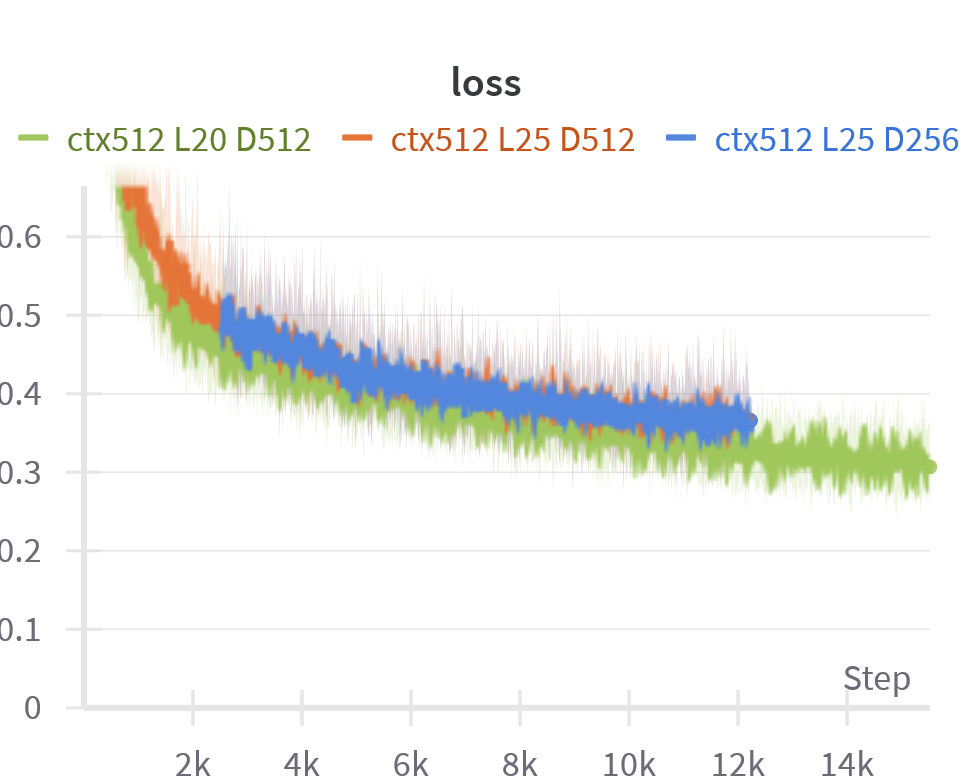
\includegraphics[width=8cm]{Figures/loss-pi.png} }}%
      \qquad
      \subfloat[تغییر نرخ یادگیری]{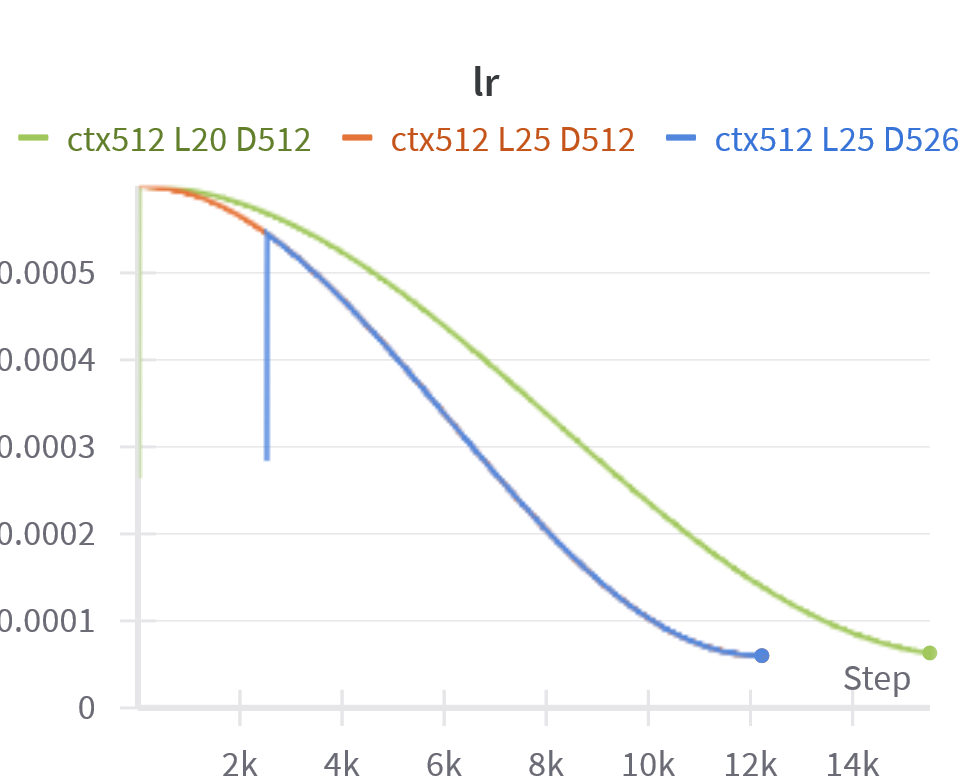
\includegraphics[width=8cm]{Figures/lr-pi.png} }%
      \caption{نمودار های پیشرفت یادگیری مدل پیانو}%
      \label{Fig:lrpi}%
\end{figure}


\subsection{ارزیابی مدل درام}
مطابق با نمودار \ref{Fig:lrdr} میتوان گفت که
مدل بنفش\footnote{در اینجا مدل بنفش به مدل  \lr{ctx512 L20 D512} اشاره می‌کند. که مدل نهایی انتخاب شده برای ارزیابی است.} با مقدار خطای اولیه کمتری شروع می‌شود و به تدریج در طول زمان کاهش می‌یابد. این نشان‌دهنده یک فرآیند یادگیری پایدار است.
کاهش تدریجی مقدار خطا نشان می‌دهد که مدل در حال یادگیری و تطبیق خوب است که این یک نشانه مثبت است. با تنظیمات بیشتر و دوره‌های آموزشی اضافی، مدل بنفش پتانسیل دستیابی به عملکرد حتی بهتر را دارد. ولی به احتمال زیاد ادامه آموزش این مدل باعث \lr{overfit} شدن خواهد شد زیرا حجم داده های دارم خیلی بالا نیست و ادامه بیش از این احتمالا باعث \lr{overfit} می شود.

\begin{figure}
      \centering
      \subfloat[تغییر مقدار تابع خطا]{{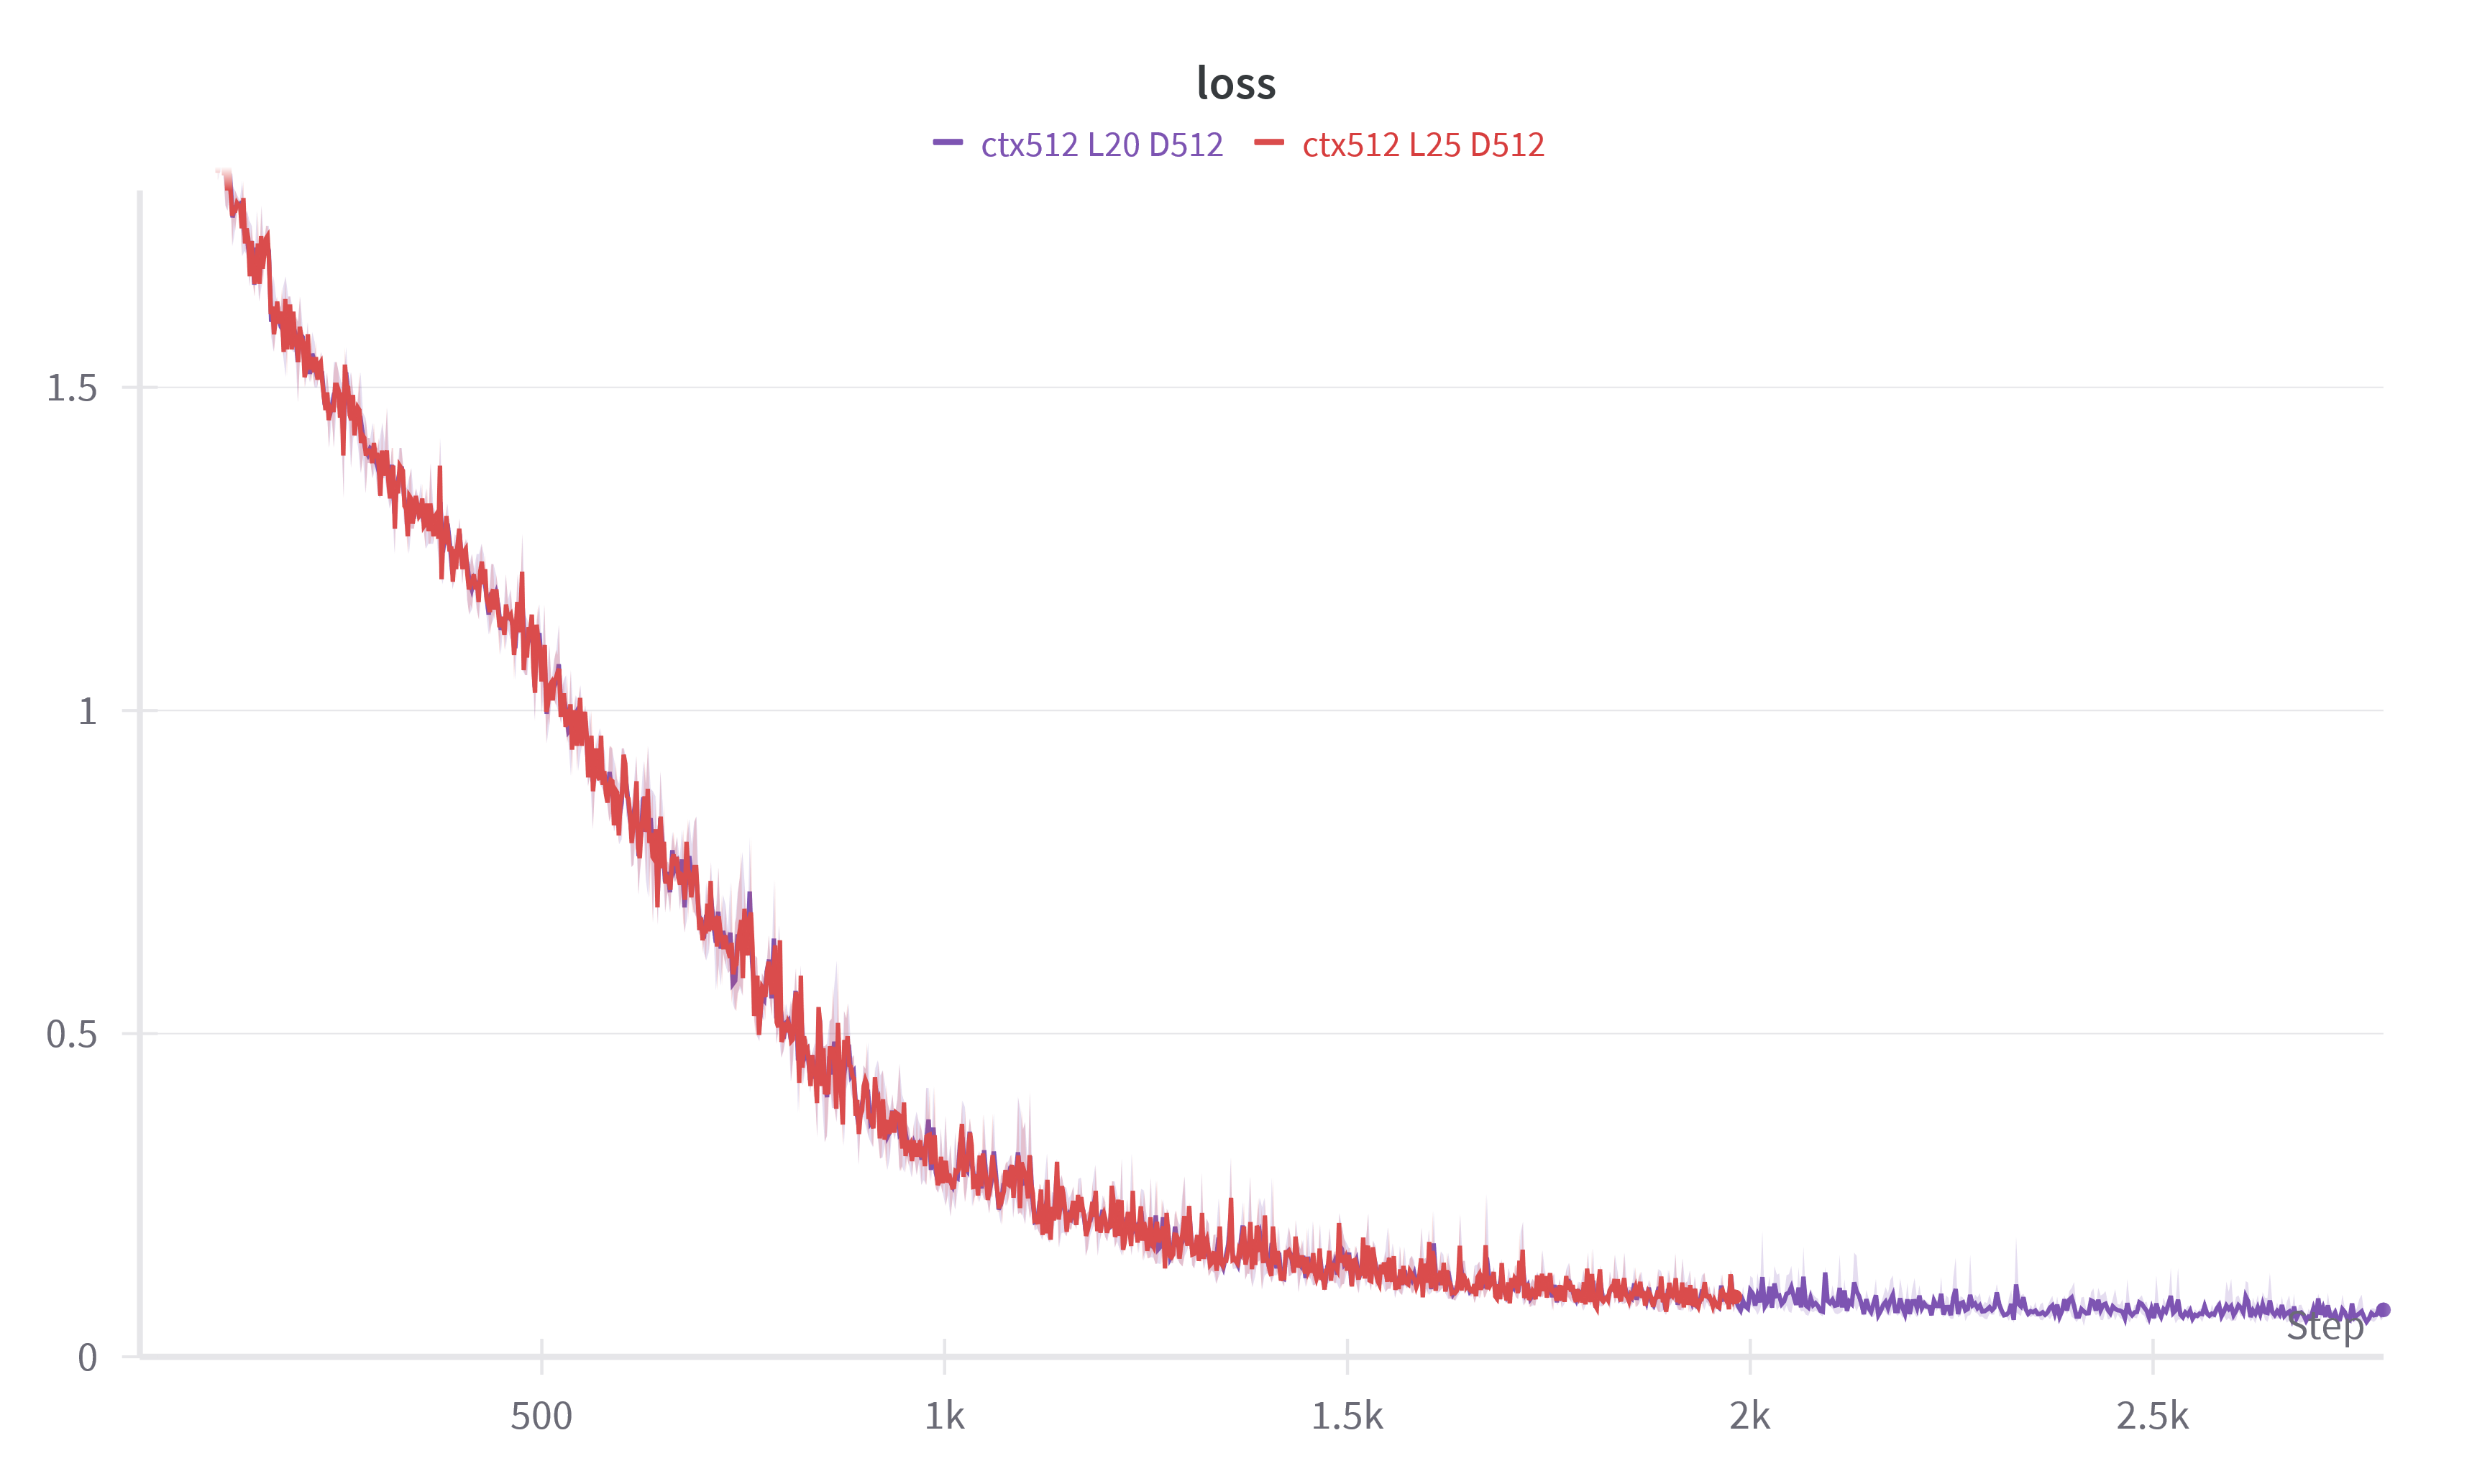
\includegraphics[width=8cm]{Figures/loss-dr.png} }}
      \qquad
      \subfloat[تغییر نرخ یادگیری]{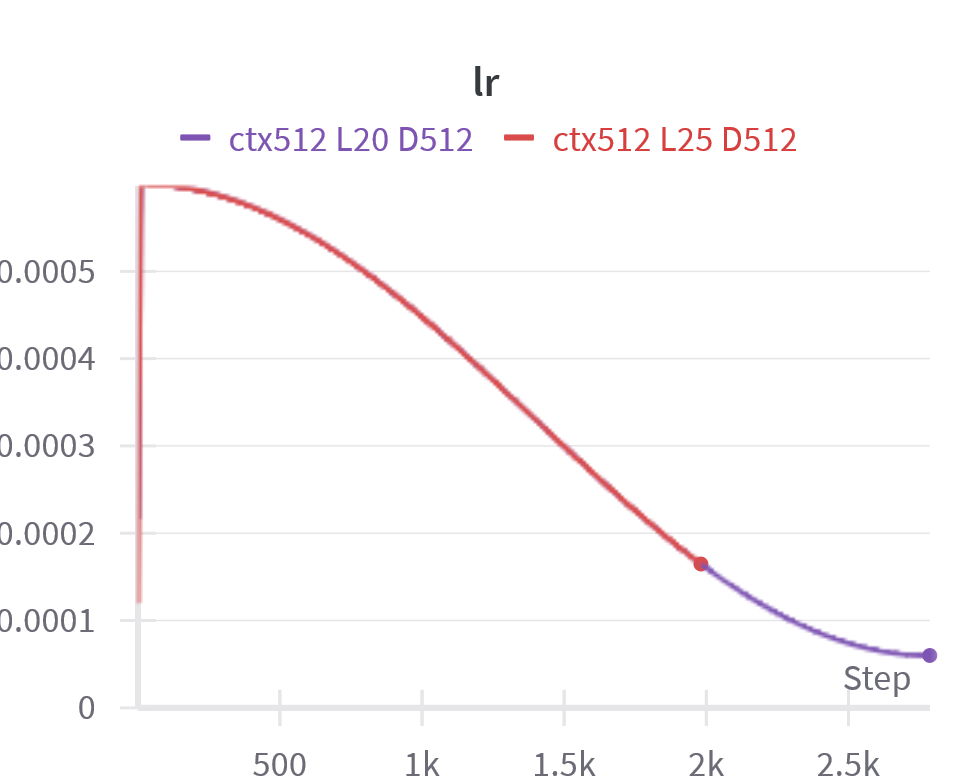
\includegraphics[width=8cm]{Figures/lr-dr.png} }
      \caption{نمودار های پیشرفت یادگیری مدل درام}
      \label{Fig:lrdr}
\end{figure}

\subsection{ارزیابی عملکرد مدل با معیار های موسیقی}

برای ارزیابی عملکرد مدل زبان کوچک ما در تولید موسیقی لو-فی، از مجموعه ای از معیارهای ارزیابی استفاده می شود که کیفیت های مختلف موسیقی مانند ریتم، ملودی و توالی را ارزیابی می کنند. بخش های زیر معیارهای مورد استفاده برای ارزیابی عملکرد مدل را به تصویر می‌کشند. اکثر این میعار ها در مقاله \lr{A Comprehensive Survey for Evaluation Methodologies of AI-Generated Music} \cite{xiong2023comprehensive} معرفی شده اند. و ما آن ها را با کتابخانه \lr{music21} \cite{conf/ismir/CuthbertA10} پیاده سازی کردیم.
\subsubsection{هماهنگی ریتم \lr{(Rhythm Consistency)}}

هماهنگی ریتم یک متریک است که به بررسی نوسان یا یکنواختی طول نت ها در یک قطعه موسیقی می پردازد. این متریک نشان می دهد که قطعه های موسیقی چه میزان یکنواختی و یا چه میزان نوسانی دارند.

فرمول و محاسبه

فرمول هماهنگی ریتم به صورت زیر است:
\begin{math}
      RC =  \frac{\mu}{\mu + SD}
\end{math}

در این فرمول:
\begin{itemize}
      \item  \lr{SD} معیار انحراف معیار طول نت ها است
      \item  ${\mu}$ میانگین طول نت ها است
\end{itemize}

\xal{alg:analyze_rhythm_consistency} نشان دهنده نحویه انجام این کار برای یک فایل \lr{MIDI} است.\footnote{\label{acualCodeRef}کد پاینون این الگوریم را میتوانید در \url{} مشاهده کنید.}

\begin{LTR}
      \begin{algorithm}
            \caption{هماهنگی ریتم}
            \setmainfont{Times New Roman}
            \label{alg:analyze_rhythm_consistency}
            \begin{algorithmic}
                  \Require {MIDI file}
                  \Ensure {rhythm consistency measure}
                  \State {Parse the MIDI file using a converter to obtain a score}
                  \State {Extract notes from the score}
                  \State {Extract durations of notes}
                  \State {Calculate the mean duration of notes}
                  \State {Calculate the variance of note durations}
                  \State {Calculate the standard deviation of note durations as the square root of the variance}
                  \State {Return the standard deviation of note durations}
            \end{algorithmic}
      \end{algorithm}
\end{LTR}

این فرمول برای نرمال سازی معیار نقطه کمره طول نت ها توسط میانگین، امکان مقایسه و تفسیر بهتر هماهنگی ریتم را فراهم می کند. نتیجه به صورت یک عدد بین 0 و 1 است:

\begin{itemize}
      \item هماهنگی ریتم = 1 نشان دهنده هماهنگی کامل (همه نت ها طول یکسانی دارند)
      \item هماهنگی ریتم = 0 نشان دهنده عدم هماهنگی کامل (نت ها طول های بسیار متفاوت دارند)
      \item هماهنگی ریتم = 0.5 نشان دهنده هماهنگی متوسط (نت ها طول هایی یکنواخت اما با کمی نوسان دارند)
\end{itemize}

\subsubsection{ شباهت ملودی \lr{(Melodic Similarity Metric)}}

متحلیل شباهت ملودی، یک متد برای اندازه گیری شباهت بین دو ملودی بر اساس ترتیب نت‌هایشان است. این متد ساده و مستقیماً از نسبت نت‌های مشابه دو ملودی برای محاسبه شباهت استفاده می‌کند.

فرمول:

شباهت ملودی = (تعداد نت‌های مشابه) / (اندازه کوتاه‌ترین ملودی)

در این فرمول:
تعداد نت‌های مشابه، تعداد نت‌هایی است که در همان موقعیت در دو ملودی وجود دارند.
اندازه کوتاه‌ترین ملودی، طول کوتاه‌ترین ملودی بین دو ملودی است.
\xal{alg:analyze_melodic_similarity} نشان دهنده نحویه انجام این کار برای یک فایل \lr{MIDI} است. \footref{acualCodeRef}

\begin{LTR}
      \begin{algorithm}
            \caption{شباهت ملودی }
            \setmainfont{Times New Roman}
            \label{alg:analyze_melodic_similarity}
            \begin{algorithmic}
                  \Require {MIDI file, Reference MIDI file}
                  \Ensure {melodic similarity measure}
                  \State {Parse the input MIDI file using a converter to obtain a score}
                  \State {Parse the reference MIDI file using a converter to obtain a reference score}
                  \State {Extract generated melody from the score}
                  \State {Extract reference melody from the reference score}
                  \State {Extract pitch sequences from the generated and reference melodies}
                  \State {Calculate the number of matching pitches between the generated and reference pitch sequences}
                  \State {Calculate the similarity as the ratio of matching pitches to the length of the shorter pitch sequence}
                  \State {Return the melodic similarity measure}
            \end{algorithmic}
      \end{algorithm}
\end{LTR}
\subsubsection{ ثبات تونال \lr{(Tonal Stability Metric)}}

متحلیل ثبات تونال، یک متد برای اندازه گیری ثبات تونال یک ملودی است. این متد از تعداد تغییرات کلید در یک ملودی برای محاسبه ثبات تونال استفاده می‌کند.

فرمول:

ثبات تونال = 1 - (تعداد تغییرات کلید)

به عبارت دیگر، هرچه تعداد تغییرات کلید در یک ملودی کمتر باشد، ثبات تونال آن بیشتر است.
\xal{alg:analyze_tonal_stability} نشان دهنده نحویه انجام این کار برای یک فایل \lr{MIDI} است.\footref{acualCodeRef}


\begin{LTR}
      \begin{algorithm}
            \caption{ثبات تونال }
            \setmainfont{Times New Roman}
            \label{alg:analyze_tonal_stability}
            \begin{algorithmic}
                  \Require {MIDI file}
                  \Ensure {tonal stability measure}
                  \State {Parse the MIDI file using a converter to obtain a score}
                  \State {Extract key changes from the score}
                  \State {Count the number of key changes}
                  \State {Return the number of key changes}
            \end{algorithmic}
      \end{algorithm}
\end{LTR}

\subsubsection{ هماهنگی هارمونیک \lr{(Harmonic Coherence Metric)} }

هماهنگی هارمونیک یک متد برای اندازه گیری هماهنگی هارمونیک یک ملودی است. این متد از نسبت هارمونی سازگار (ملایمت) و غیرسازگار (نا‌هم‌خوانی) در یک ملودی برای محاسبه هماهنگی هارمونیک استفاده می‌کند.

فرمول:

هماهنگی هارمونیک = (نسبت ملایمت + نسبت نا‌هم‌خوانی)

نسبت ملایمت: نسبت تعداد هارمونی‌های سازگار به کل تعداد هارمونی‌ها
نسبت دیشنانسه: نسبت تعداد هارمونی‌های غیرسازگار به کل تعداد هارمونی‌ها

به عبارت دیگر، هرچه نسبت ملایمت در یک ملودی بیشتر باشد، هماهنگی هارمونیک آن بیشتر است.
\xal{alg:harmonicCoherence} نشان دهنده نحویه انجام این کار برای یک فایل \lr{MIDI} است.\footref{acualCodeRef}

\begin{LTR}
      \begin{algorithm}
            \caption[هماهنگی هارمونیک]{هماهنگی هارمونیک}
            \setmainfont{Times New Roman}
            \label{alg:harmonicCoherence}
            \begin{algorithmic}[1]
                  \Procedure{analyzeHarmonicCoherence}{midi\_file}
                  \State Parse MIDI file: $score \leftarrow converter.parse(midi\_file)$
                  \State Analyze key: $key\_analysis \leftarrow score.analyze('key')$
                  \State Chordify score: $chords \leftarrow score.chordify()$
                  \State Get chord list: $chord\_list \leftarrow [ch \text{ for } ch \text{ in } chords.recurse().Chord]$
                  \State Count consonant chords:
                  \State $consonance\_count \leftarrow \sum_{ch \in chord\_list} 1 \text{ if } ch.isConsonant() \text{ else } 0$
                  \State Calculate ratios: $dissonance\_count \leftarrow \text{len}(chord\_list) - consonance\_count$
                  \State $total\_chords \leftarrow \text{len}(chord\_list)$
                  \State $consonance\_ratio \leftarrow consonance\_count / total\_chords$
                  \State $dissonance\_ratio \leftarrow dissonance\_count / total\_chords$
                  \State \Return $consonance\_ratio, dissonance\_ratio$
                  \EndProcedure
            \end{algorithmic}
      \end{algorithm}
\end{LTR}
برای کد های الگوریتم های گفته می‌توانید به \ref{ap:codes} مراجعه کنید.
\subsubsection{نتایج این معیار ها برای مدل پیانو}
\begin{table}
      \centering
      \caption{نتایج این معیار ها برای مدل پیانو}
      \label{resultPi}
      \begin{tabular}{|l|l|}
            \hline
            متد                          & مقدار \\ \hline
            هماهنگی ریتم                 & 0.34  \\ \hline
            هماهنگی هارمونیک (ملایمت)    & 0.87  \\ \hline
            هماهنگی هارمونیک (نا‌هم‌خوانی) & 0.13  \\ \hline
            تغییرات کلید                 & 0.2   \\ \hline
      \end{tabular}
\end{table}
تحیل  \xt{resultPi} به صورت زیر است:
\begin{itemize}
      \item[هماهنگی ریتم] مقدار 0.34 نشان‌دهنده این است که ریتم ملودی دارای تناوب‌های نسبتاً مشابه است، اما همچنان دارای برخی از تغییرات و نوسانات است.
      \item[هماهنگی هارمونیک] مقدار 0.87 نشان‌دهنده این است که هارمونی‌های ملودی در مجموع سازگار هستند و دارای هماهنگی بالایی هستند.
      \item[تغییرات کلید] مقدار 0.2 نشان‌دهنده این است که ملودی تقریبا هیچ تغییراتی در کلید ندارد و در کلید ثابت باقی می‌ماند.
\end{itemize}

ملودی های ساخته شده توسط مدل دارای هماهنگی بالایی در هارمونی و ریتم است، اما هنوز دارای بعضی از ناهمسانی‌ها و عدم هماهنگی است که می تواند بهبود یابد.

\section{ساخت موسیقی نهایی}\label{finalMusic}
در کد ما که در \xal{algo:lofi_music} نشان داده شده است، برای تولید موسیقی لو-فای، چندین روش به کار گرفته شده است
تا یک قطعه موسیقی منحصر به فرد و هماهنگ ایجاد شود. این فرآیند با تولید
یک تمپوی تصادفی آغاز می‌شود که به هر قطعه موسیقی تنوع و یگانگی می‌بخشد.
هسته اصلی تولید موسیقی شامل تبدیل خروجی مدل به فایل‌های \lr{MIDI} با استفاده
از تابع \texttt{convert\_str\_to\_midi} است که مربوط به بخش \ref{se:tokenizer} است که در \xal{al:tokenMidi} و \xal{al:strMidi} نشان داده شده است. این فایل‌های \lr{MIDI} سپس با
استفاده از \lr{FluidSynth}، یک نرم‌افزار سینتی‌سایزر که برای تولید صدا به
فونت‌های صوتی متکی است، به فایل‌های صوتی تبدیل می‌شوند. فونت‌های صوتی، مانند
فونت مشخص شده در کد ما
(\texttt{SGM-v2.01-NicePianosGuitarsBass-V1.2.sf2})، مجموعه‌ای از
نمونه‌های صوتی هستند که صدای سازهای واقعی و با کیفیت بالا را فراهم
می‌کنند. این امر برای موسیقی لو-فای بسیار مهم است، زیرا بافت و طنین سازها
به طور قابل توجهی به زیبایی کلی موسیقی کمک می‌کند.

\begin{LTR}
      \begin{algorithm}
            \caption{تبدیل توکن به \lr{MIDI}}
            \label{al:tokenMidi}
            \setmainfont{Times New Roman}
            \begin{algorithmic}[1]
                  \State \textbf{Input:} utils, token, state, channel, end\_token\_pause
                  \State \textbf{Output:} Iterator of (Optional MIDI Message, DecodeState)

                  \If{state is None}
                  \State Initialize state
                  \EndIf

                  \State token $\leftarrow$ token.strip()

                  \If{token is empty or starts with "<"}
                  \State yield (None, state)
                  \Return
                  \EndIf

                  \If{token is "<end>"}
                  \State Update state with end\_token\_pause
                  \If{utils.cfg.decode\_end\_held\_note\_delay $\neq$ 0.0}
                  \For{(channel, note), start\_time in state.active\_notes}
                  \State Convert delta\_accum to ticks
                  \State Remove (channel, note) from active\_notes
                  \State yield (note\_off message, state)
                  \EndFor
                  \EndIf
                  \State yield (None, state)
                  \Return
                  \EndIf

                  \If{token is a wait token}
                  \State Update state with wait token delta
                  \If{utils.cfg.decode\_end\_held\_note\_delay $\neq$ 0.0}
                  \For{(channel, note), start\_time in state.active\_notes}
                  \If{note held too long}
                  \State Convert delta\_accum to ticks
                  \State Remove (channel, note) from active\_notes
                  \State yield (note\_off message, state)
                  \Return
                  \EndIf
                  \EndFor
                  \EndIf
                  \Else
                  \State (bin, note, velocity) $\leftarrow$ utils.note\_token\_to\_data(token)
                  \State Convert delta\_accum to ticks
                  \If{velocity $>$ 0}
                  \If{utils.cfg.decode\_fix\_repeated\_notes and (channel, note) in active\_notes}
                  \State Remove (channel, note) from active\_notes
                  \State yield (note\_off message, state)
                  \EndIf
                  \State Add (channel, note) to active\_notes
                  \State yield (note\_on message, state)
                  \Else
                  \State Remove (channel, note) from active\_notes
                  \State yield (note\_off message, state)
                  \EndIf
                  \EndIf

                  \State yield (None, state)
            \end{algorithmic}
      \end{algorithm}

      \begin{algorithm}
            \setmainfont{Times New Roman}
            \caption{متن به \lr{MIDI message}}
            \label{al:strMidi}
            \begin{algorithmic}[1]
                  \State \textbf{Input:} utils, data, channel
                  \State \textbf{Output:} Iterator of MIDI Messages

                  \State state $\leftarrow$ None

                  \For{token in data.split(" ")}
                  \For{msg, new\_state in token\_to\_midi\_message(utils, token, state, channel)}
                  \State state $\leftarrow$ new\_state
                  \If{msg is not None}
                  \State yield msg
                  \EndIf
                  \EndFor
                  \EndFor

            \end{algorithmic}
      \end{algorithm}
\end{LTR}

استفاده از فونت‌های صوتی چندین مزیت دارد. آن‌ها صدای سازهای واقعی را فراهم
می‌کنند که اصالت موسیقی تولید شده را افزایش می‌دهد. همچنین امکان
سفارشی‌سازی را فراهم می‌کنند و به شما اجازه می‌دهند فونت‌های صوتی را انتخاب
کنید که با سبک و احساس مورد نظر موسیقی مطابقت داشته باشند. یکنواختی در
کیفیت صدا نیز یکی دیگر از مزایا است که اطمینان می‌دهد موسیقی دارای صدای
یکنواختی است. علاوه بر این، فونت‌های صوتی فرآیند سینتی‌سایز را کارآمد
می‌کنند، زیرا \lr{FluidSynth} نمونه‌های صوتی از پیش ضبط شده را طبق
دستورالعمل‌های \lr{MIDI} پخش می‌کند.

پس از تبدیل فایل‌های \lr{MIDI} به فایل‌های صوتی، ما از \texttt{pydub} برای
بارگذاری و دستکاری این قطعات صوتی استفاده می‌کند. این شامل رول پیانو
اصلی، لوپ‌های درام که توسط مدل های ما ساخته شده است و  \lr{sfx sound} است. یک \lr{sfx sound} تصادفی انتخاب می‌شود
تا به موسیقی بافت و تصادفی بودن اضافه کند. توالی درام به طور مشابه با
ملودی اصلی پردازش می‌شود تا هماهنگی با موسیقی تولید شده را تضمین کند.
قطعات صوتی مختلف سپس برای ایجاد لایه‌دار روی هم قرار
می‌گیرند. حجم رول پیانو تنظیم می‌شود و لوپ‌های \lr{sfx sound} و درام برای مطابقت با
مدت زمان رول پیانو تکرار می‌شوند. قطعه موسیقی نهایی با تکرار قطعات مخلوط
شده به طول مورد نظر گسترش می‌یابد و با یک افکت محو شدن در پایان، یک پایان
نرم ایجاد می‌شود. برای دسترسی به کد ها و اجرا آنها به \xa{ap:codes} مراجعه کنید.

\begin{LTR}
      \begin{algorithm}[H]
            \caption{نحویه ساخت موسیقي نهایی}
            \label{algo:lofi_music}
            \setmainfont{Times New Roman}
            \begin{algorithmic}[1]
                  \Procedure{GenMusic}{data, dataDrum}
                  \State $tempo \gets \text{random.randint(14, 18) \* 5}$ \Comment{Set tempo}
                  \State $\text{convert\_str\_to\_midi}(\text{\_\_join}(data), tempo) \gets \text{save}(\text{relpath}(\text{./soundFont/mdiOut.mid}))$ \Comment{Generate MIDI file}
                  \State $\text{fs} \gets \text{FluidSynth}(\text{relpath}(\text{./soundFont/SGM-v2.01-NicePianosGuitarsBass-V1.2.sf2}))$ \Comment{Load sound font}
                  \State $\text{fs.midi\_to\_audio}(\text{relpath}(\text{./soundFont/mdiOut.mid}), \text{relpath}(\text{./soundFont/output.flac}))$ \Comment{Convert MIDI to audio}
                  \State $\text{pianoRoll} \gets \text{AudioSegment.from\_file}(\text{relpath}(\text{./soundFont/output.flac}))$ \Comment{Load piano roll}
                  \State $\text{fillName} \gets \text{random.choice}(\text{os.listdir}(\text{relpath}(\text{./loops/vinyl})))$ \Comment{Select fill name}
                  \State $\text{fill} \gets \text{AudioSegment.from\_file}(\text{relpath}(\text{./loops/vinyl/}\text{fillName}))$ \Comment{Load fill}
                  \State $\text{convert\_str\_to\_midi}(\text{\_\_join}(data), 400, 9) \gets \text{save}(\text{relpath}(\text{./soundFont/mdiOutDrum.mid}))$ \Comment{Generate drum MIDI file}
                  \State $\text{fs.midi\_to\_audio}(\text{relpath}(\text{./soundFont/mdiOutDrum.mid}), \text{relpath}(\text{./soundFont/output.flac}))$ \Comment{Convert drum MIDI to audio}
                  \State $\text{drum} \gets \text{AudioSegment.from\_file}(\text{relpath}(\text{./soundFont/output.flac}))$ \Comment{Load drum}
                  \EndProcedure

                  \Procedure{mix\_lines}{music\_len}
                  \State $\text{pianoRoll} \gets \text{pianoRoll} + 10$ \Comment{Adjust piano roll}
                  \State $\text{fill} \gets \text{fill} \* \text{math.ceil}(\text{pianoRoll.duration\_seconds} / \text{fill.duration\_seconds})$ \Comment{Repeat fill}
                  \State $\text{drum} \gets \text{drum} \* \text{math.ceil}(\text{pianoRoll.duration\_seconds} / \text{drum.duration\_seconds})$ \Comment{Repeat drum}
                  \State $\text{music} \gets \text{pianoRoll}\text{.overlay}(\text{fill} - 10)\text{.overlay}(\text{drum} + 3)$ \Comment{Mix audio}
                  \State $\text{music} \gets \text{music} \* \text{math.ceil}(\text{music\_len} / \text{music.duration\_seconds})$ \Comment{Repeat music}
                  \State $\text{music} \gets \text{music.fade\_out}(2 \* \text{SECOND})$ \Comment{Fade out music}
                  \State \Return $\text{music}$
                  \EndProcedure
            \end{algorithmic}
      \end{algorithm}
\end{LTR}